\subsection{CU10 Visualizar Empleados}
Cuando el administrador selecciona la opción 'Gestionar Empleados' del menú (figura \ref{fig:Pantalla Visualizar Menu Administrador - Vista de Escenarios}) aparece en pantalla la siguiente ventana. En ella se podrán visualizar a todos los empleados que están registrados dentro de la base de datos y que, obviamente, están trabajando dentro del taller. En la parte inferior de la ventana, existen más botones.
\begin{itemize}
	\item \textbf{Actualizar Registros:} Cuando se haga una acción en alguno de los registros, es necesario presionar este botón para que se actualicen todos los datos de la tabla-
	\item \textbf{Registrar Empleado:} Cuando se presiona este botón aparece una nueva ventana donde se podrá ingresar los datos de un nuevo empleado.
	\item \textbf{Modificar Empleado:} Al seleccionar una fila de la tabla (a un empleado registrado), aparecerá una ventana con un formulario de actualización.
	\item \textbf{Eliminar Empleado:} Al seleccionar una fila de la tabla (empleado registrado), aparecerá una ventana con un mensaje de seguridad para verificar si realmente se desea eliminar ese registro.
	\item \textbf{Salir:} El administrador cierra esa ventana y al mismo tiempo regresa al menú, figura \ref{fig:Pantalla Visualizar Menu Administrador - Vista de Escenarios}.
\end{itemize}
\begin{figure}[!h]
	\centering
	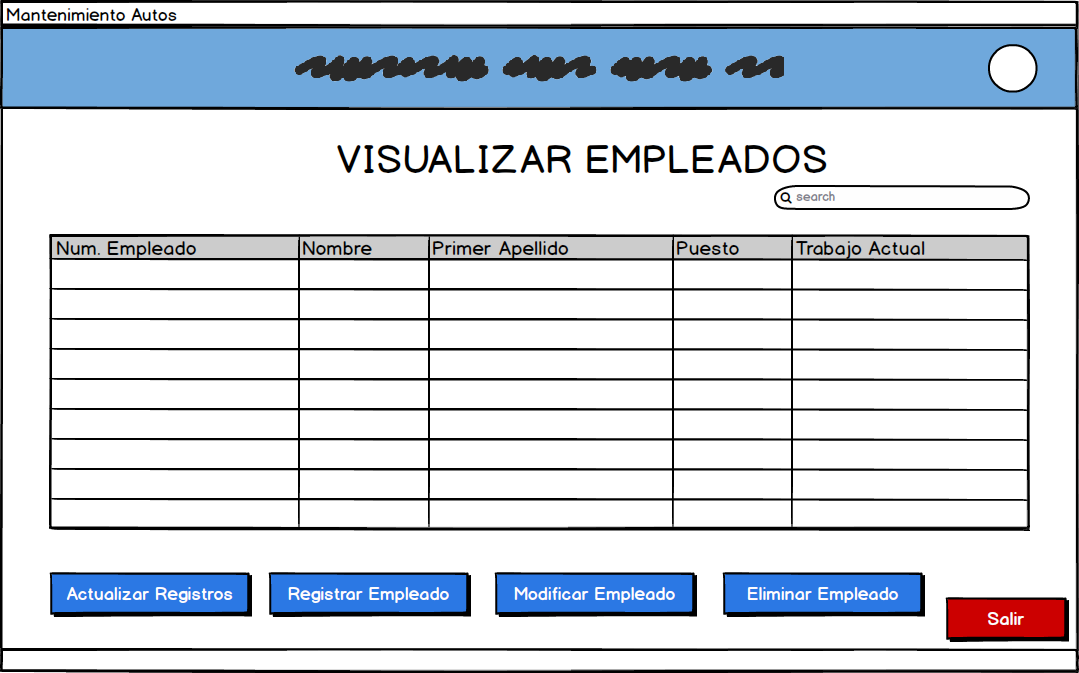
\includegraphics[width=1\textwidth]{./diseno/vescenarios/imagenes/VisualizarEmpleados}
	\caption{Pantalla Visualizar Empleados - Vista de Escenarios}
	\label{fig:Pantalla Visualizar Empleados - Vista de Escenarios}
\end{figure}
En dado caso de que se quiera modificar o eliminar un registro y no se ha seleccionado un renglón de la tabla, aparecerá un mensaje de alerta que le dirá al administrador que debe de seleccionar un registro.
\begin{figure}[!h]
	\centering
	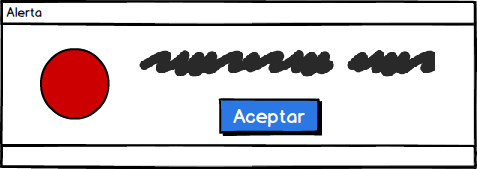
\includegraphics[width=0.5\textwidth]{./diseno/vescenarios/imagenes/alerta}
	\caption{Alerta - Vista de Escenarios}
	\label{fig:Alerta Empleados - Vista de Escenarios}
\end{figure}
\clearpage